\subsection{Monotonicity and extrema on the graph}

The cubic
\[
f(x)=x^3-3x
\]
has a local maximum at $x=-1$ and a local minimum at $x=1$. These points divide the graph into increasing and decreasing intervals.

\begin{center}
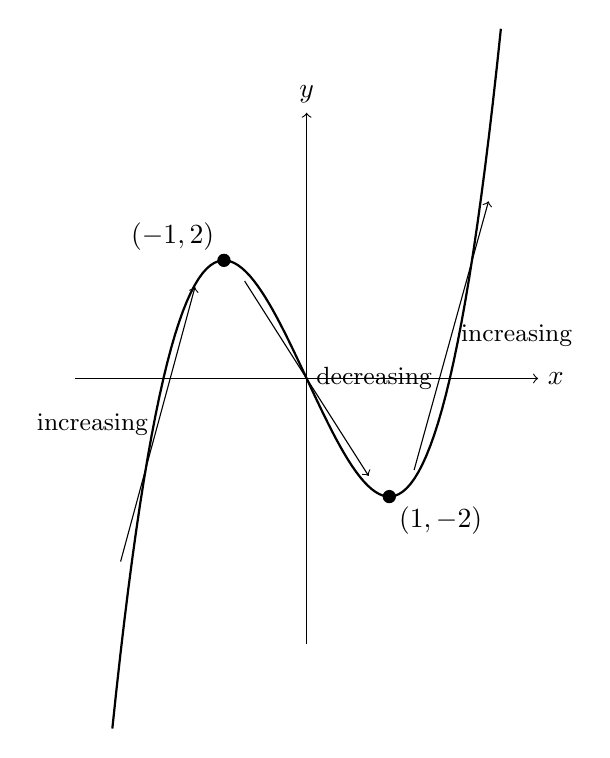
\begin{tikzpicture}[x=1.05cm,y=0.75cm]
  \draw[->] (-2.8,0) -- (2.8,0) node[right] {$x$};
  \draw[->] (0,-4.5) -- (0,4.5) node[above] {$y$};
  \draw[thick,domain=-2.35:2.35,samples=100] plot (\x,{\x*\x*\x-3*\x});
  \fill (-1,2) circle (2.4pt) node[above left] {$(-1,2)$};
  \fill (1,-2) circle (2.4pt) node[below right] {$(1,-2)$};
  \draw[->] (-2.25,-3.1) -- (-1.35,1.55) node[midway,left] {\small increasing};
  \draw[->] (-0.75,1.65) -- (0.75,-1.65) node[midway,right] {\small decreasing};
  \draw[->] (1.3,-1.55) -- (2.2,3.0) node[midway,right] {\small increasing};
\end{tikzpicture}
\end{center}

\begin{interpretationbox}[A critical point must be classified]
The derivative is zero at both marked points, but the sign change determines the type: positive to negative gives a local maximum, while negative to positive gives a local minimum.
\end{interpretationbox}
